\title{Final Exam}
\author{Dr. Jordan Hanson - Whittier College Dept. of Physics and Astronomy}
\date{\today}
\documentclass[10pt]{article}
\usepackage[a4paper, total={18cm, 27cm}]{geometry}
\usepackage{outlines}
\usepackage{graphicx}
\begin{document}
\maketitle

\section{Chapter 1 - Introductory Concepts}

\begin{enumerate}
\item Suppose we have a parallel data stream of 4-bits.  Each clock cyle, 4 bits are recieved.  The clock period is 0.1 microseconds.  How many bits per second are being transmitted? \\ \vspace{1cm}
\item A system sends digital pulses with pulse widths of 20 ns at a frequency of 10 MHz.  What is the duty cycle of these pulses? \\ \vspace{1cm}
\item \textbf{Special topics: ADCs}  If an ADC input range goes from 0.0 to 2.5 Volts, and digitizes analog voltages into 8-bit binary numbers, what is the smallest change in voltage the system could detect? \\ \vspace{1cm}
\end{enumerate}

\section{Chapter 2 - Number Systems and Codes}

\begin{enumerate}
\item (a) How many bits are necessary to create binary numbers to represent each letter of the alphabet with one number (26 letters)? (b) Write your first name, but encoded letter by letter in binary. \\ \vspace{1cm}
\item Repeat the prior exercise with hexedecimal numbers instead of binary ones.  \\ \vspace{1cm}
\end{enumerate}

\section{Chapter 3 - Logic Gates}

\begin{figure}
\centering
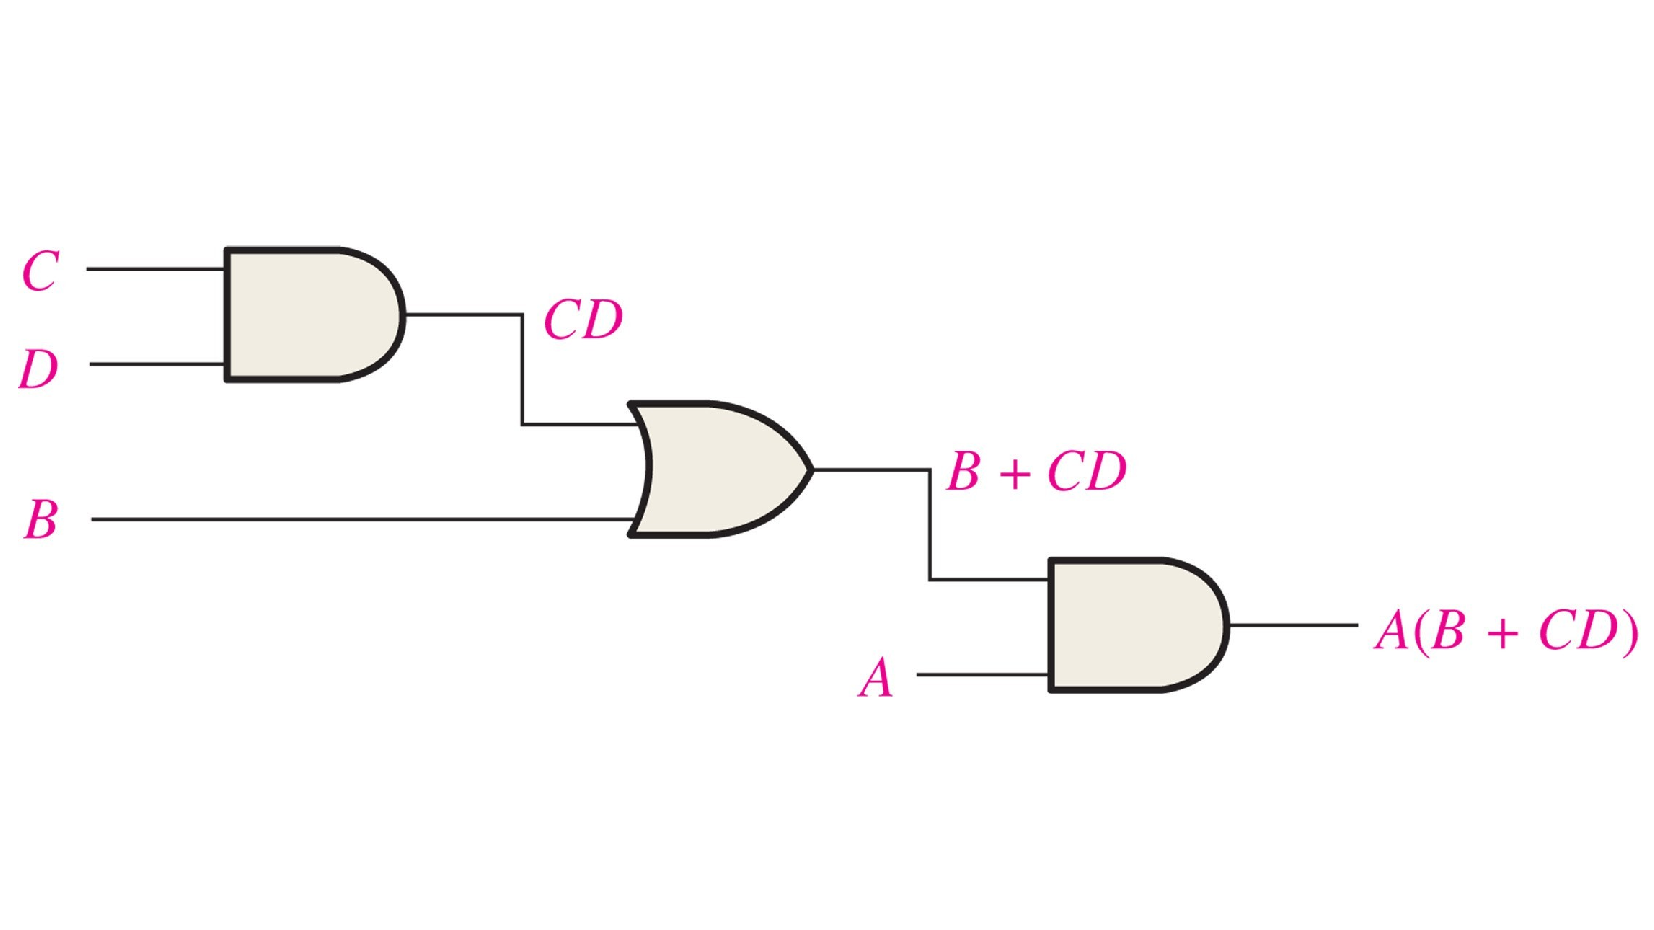
\includegraphics[width=0.4\textwidth,trim=0cm 3cm 0cm 3cm,clip=true]{figures/final1.pdf}
\caption{\label{fig:final1} Example circuit for chapter 3.}
\end{figure}

\begin{enumerate}
\item (a) In a certain manufacturing process, electrical components are automatically placed on a printed ciruit board (PCB).  Before insertion, the tool must have the correct x-coordinate, y-coordinate, and the component must be ready.  Each condition is a HIGH, and the inserter proceeds on LOW.  Design a circuit that implements this process. (b) Suppose the inserter replaces $A$ in Fig. \ref{fig:final1} with $AD$.  What is the new \textit{simplified} logic function?  \\ \vspace{1cm}
\end{enumerate}

\section{Chapter 4 - Boolean Algebra and Logic Simplification}

\begin{enumerate}
\item Map the expression $X = A + \bar{C}D + AC\bar{D} + \bar{A}BC\bar{D}$ onto a Karnaugh map, group the true states, and develop the simplified logic expression for the output $X$. \\ \vspace{2cm}
\end{enumerate}

\section{Chapter 5 - Combinational Logic Analysis}

\begin{figure}
\centering
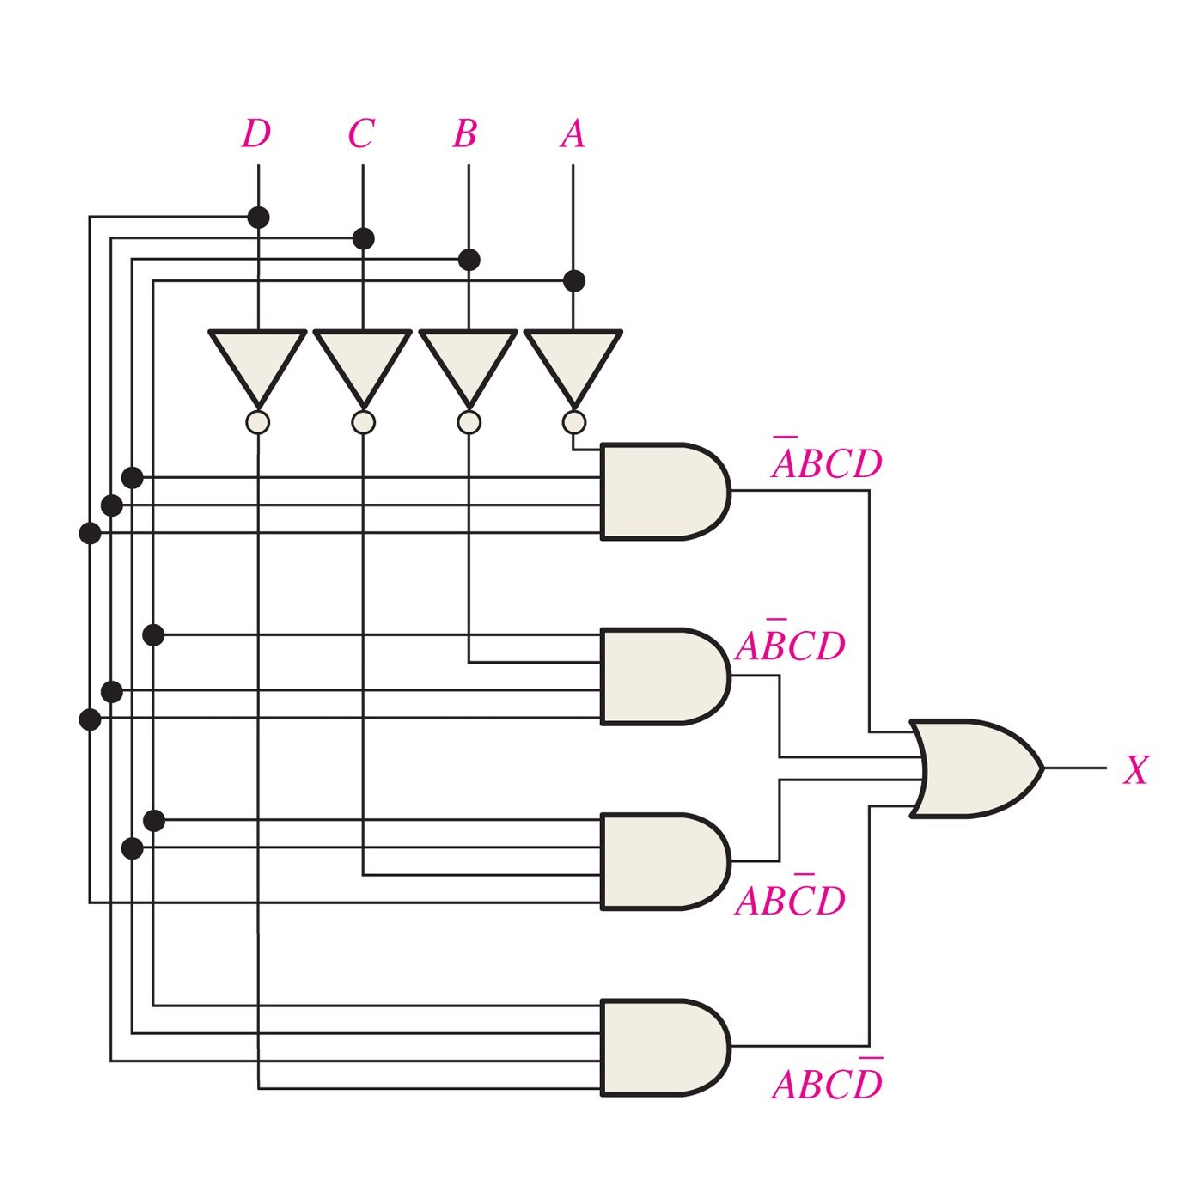
\includegraphics[width=0.45\textwidth]{figures/final2.pdf}
\caption{\label{fig:final2} Example circuit for chapter 5.}
\end{figure}

\begin{enumerate}
\item In Fig. \ref{fig:final2}, a logic function is shown that outputs 1 if exactly three inputs are 1.  (a) Develop the truth table (true states only). (b) Determine if it can be simplified. \\ \vspace{2cm}
\end{enumerate}

\section{Chapter 6 - Functions of Combinational Logic}

\begin{enumerate}
\item Suppose you have a \textit{counter} that accepts a clock signal as input, and has two outputs that cycle between 00, 01, 10, and 11.  (a) Draw a circuit connecting the 2-bit counter to the data select lines of a 1-to-4 demultiplexer.  (b) Now connect also the counter output to a 2-bit \textit{parity checker} (XOR gate), and let the output of the parity checker be the data input to the demultiplexer.  (c) What is the output timing diagram for the four demultiplexer outputs? \\ \vspace{4cm}
\end{enumerate}

\section{Chapter 7 - Latches, Flip-flops, and Timers}

\begin{figure}
\centering
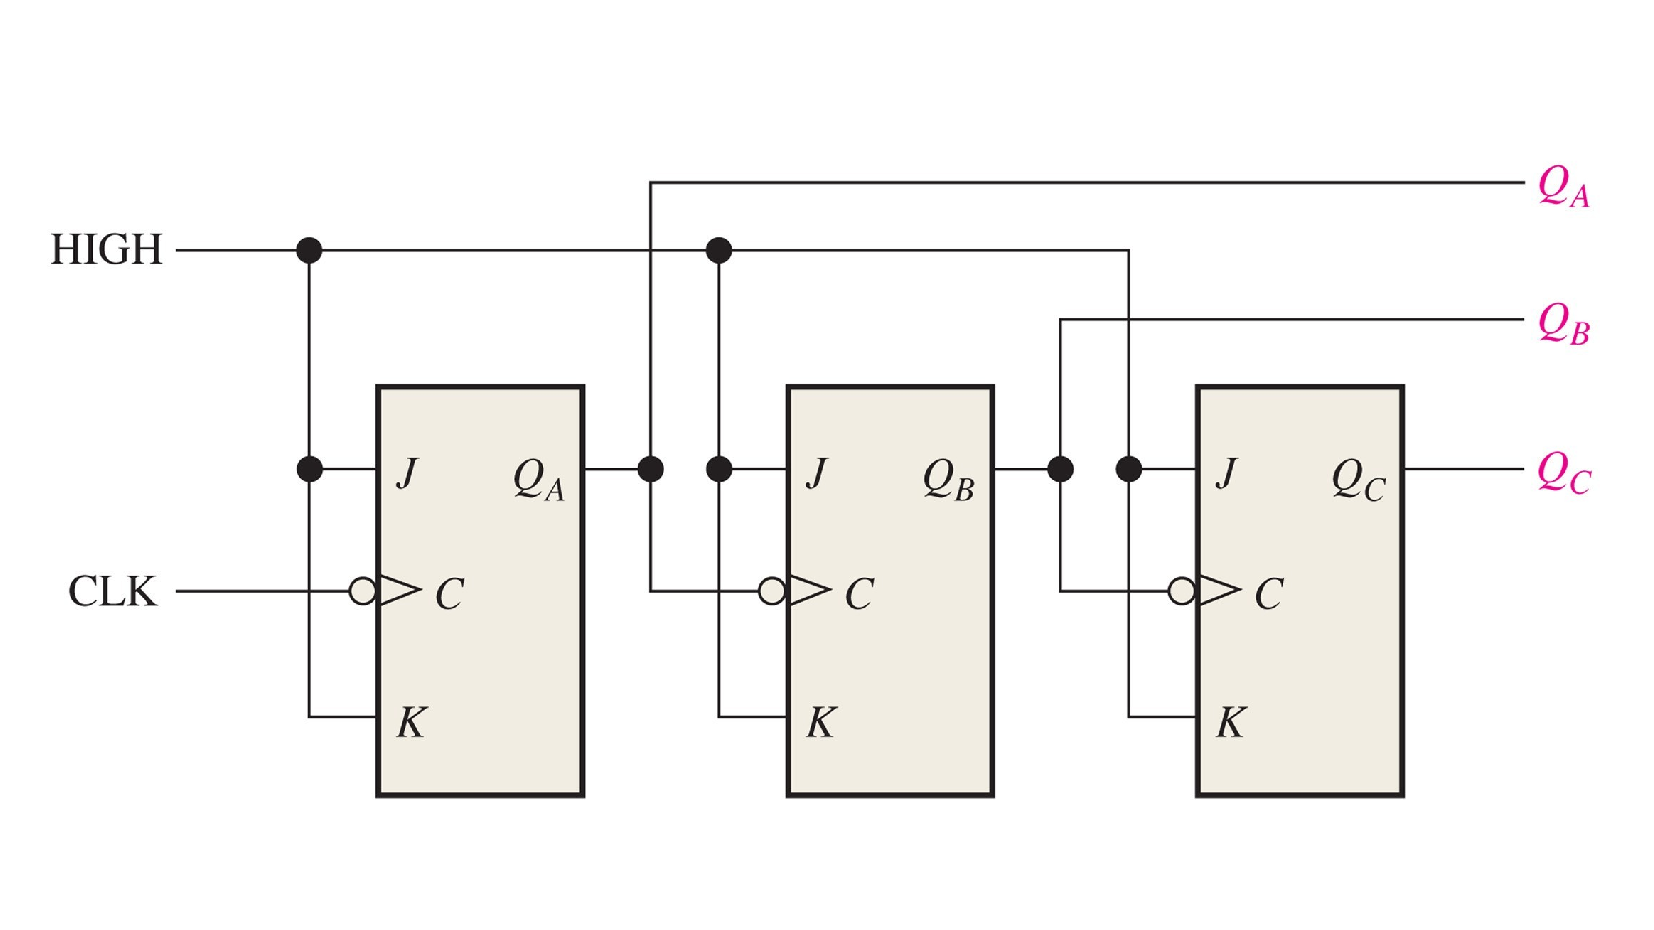
\includegraphics[width=0.55\textwidth]{figures/final3.pdf}
\caption{\label{fig:final3} Example circuit for chapter 7.}
\end{figure}

\begin{enumerate}
\item Remember the \textit{counter} mentioned in the previous problem?  Consider Fig. \ref{fig:final3}.  Determine the output waveforms in relation to the clock for $Q_A$, $Q_B$, and $Q_C$, and show that $Q_C Q_B Q_A$ is the binary sequence. \\ \vspace{3cm}
\end{enumerate}

\section{Special Topics}

\begin{enumerate}
\item \textbf{Two bonus points:} Determine the Fourier series for the sawtooth wave, which is just $f(x) = x$ from 0 to 2$\pi$, after which it goes back to zero and repeats itself.
\end{enumerate}


\end{document}